\chapter{ТАНИХ СИСТЕМИЙН АРГА ЗҮЙ}
\section{Системийн ерөнхий бүтэц}
Систем нь Зураг~\ref{fig:pipeline}-д үзүүлсэн таван алхамтай: (1) YOLO11n илрүүлэгч кадраас дугаарын хайрцгийг олно; (2) хайрцгийн өргөн/өндөр харьцаагаар нэг эсвэл хоёр мөрт гэж ангилж, хоёр мөртийг дээд ба доод мөр болгон хуваана; (3) CRNN+CTC уншигч мөр бүрийг текст болгоно; (4) дугаарын дүрэм текстийг нормчилж, хүчинтэй эсэх ба магадлалын оноог тооцно; (5) бичлэгийн хувьд IoU мөрдөлт ба итгэлээр жинлэсэн тэмдэгт тус бүрийн саналаар мөр бүрийн санал нэгдсэн дугаарыг гаргана. Хэрэгжүүлэлт \texttt{mn\_alpr} багцад байна: \texttt{charset.py}, \texttt{plate\_rules.py}, \texttt{crnn.py}, \texttt{pipeline.py}.
\begin{figure}[H]\centering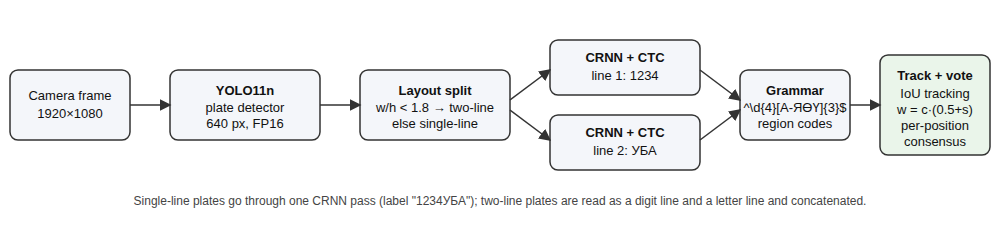
\includegraphics[width=\textwidth]{pipeline.png}
\caption{Системийн боловсруулалтын урсгал. Нэг мөрт дугаар уншигчаар нэг удаа (\plate{1234УБА}), хоёр мөрт дугаар тооны мөр ба үсгийн мөр гэж хоёр удаа орж залгагдана.}\label{fig:pipeline}\end{figure}

\section{Дугаар илрүүлэгч: YOLO11n}
Ultralytics YOLO11n~\cite{yolo11} (2.60 сая параметр, 640~px оролт, 1 анги) загварыг COCO жингээс эхлүүлж хоёр үе шаттай сургав. COCO-ийн 80 ангид дугаар байхгүй тул бэлэн жин дугаар илрүүлэхгүй; иймд \textbf{A үе}: 8\,823 олон улсын зураг дээр 25 эпох --- дугаарын ерөнхий геометрийг сурна; \textbf{B үе}: ерөнхий сургалтын 6\,176 зураг + монгол 48 зураг (hard link-ээр 15 дахин давтаж 720 болгосон) дээр 60 эпох, lr$_0=0.005$ --- монгол дугаарын хайрцгийг нарийн тохируулна. Шалгалт (загвар сонголт) монгол 18 зураг дээр mAP$_{50\text{--}95}$-аар. Нийтлэг тохиргоог Хүснэгт~\ref{tab:dethp}-д үзүүлэв; хэвтээ тусгалыг унтраасан, учир нь дугаарын үсэг толин тусгал болж буруу жишээ үүсгэнэ.
\begin{table}[H]\centering\caption{YOLO11n илрүүлэгчийн сургалтын тохиргоо}\label{tab:dethp}\small
\resizebox{\textwidth}{!}{\begin{tabular}{ll}\toprule
Параметр & Утга\\\midrule
Загвар, эхлэл & YOLO11n, COCO урьдчилан сургасан жин\\
Оролт, batch & 640~px, 32\\
Эпох & A үе 25, B үе 60 (хамгийн сайн эпох 53)\\
Сургалтын хурд & A: Ultralytics анхдагч (lr$_0$ 0.01, warmup 3 эпох); B: lr$_0$ 0.005; cosine бууралт\\
Оптимизатор & Ultralytics auto (SGD/AdamW), weight decay $5\cdot10^{-4}$\\
Алдагдлын жин & box 7.5, cls 0.5, dfl 1.5\\
Аугментаци & mosaic (сүүлийн 10 эпохд унтраана), mixup 0.1, degrees 5, shear 3, perspective 0.0005, HSV анхдагч, \textbf{fliplr 0}\\
Монгол зургийн давталт & 15$\times$ (B үе)\\
Загвар сонголт & монгол шалгалтын mAP$_{50\text{--}95}$\\\bottomrule
\end{tabular}}\end{table}

\section{Хэлбэр тодорхойлох ба мөр хуваах}
Илэрсэн хайрцгийг өргөний 3 хувь, өндрийн 6 хувиар тэлж тайрна. Өргөн/өндөр $<1.8$ бол хоёр мөрт гэж үзэж дээд 55 хувь ба доод 55 хувийг (10 хувь давхцалтай) тусад нь уншиж, тоо + үсэг гэж залгана; үгүй бол бүтнээр нь уншина. Босгыг Зураг~\ref{fig:aspect}-ийн тархалтаас сонгосон.

\section{Уншигч: CRNN + CTC}
Уншигчийн архитектур (Хүснэгт~\ref{tab:crnn}) нь Shi нарын CRNN~\cite{shi2017crnn} ба PaddleOCR-ийн уншигчийн зарчмыг дагасан: residual CNN суурь, хоёр давхар BiLSTM хүзүү, CTC толгой. Оролт: BGR мөр зургийг өндөр 48~px болгож, харьцаа хадгалан өргөнийг 192~px-ээс ихгүй болгоод баруун талд саарал (127) дүүргэж, $[-1,1]$ мужид нормчилно. Тэмдэгтийн олонлог: 10 орон + монгол кирилл 35 үсэг (\texttt{АБВГДЕЁЖЗИЙКЛМНОӨПРСТУҮФХЦЧШЩЪЫЬЭЮЯ}) + CTC blank = 46 анги. Бүх 35 үсгийг оруулсан нь ховор серийн үсгийг дүрслэх боломж олгох бөгөөд аймгийн кодын магадлалыг дүрмийн шат хариуцна. Декод greedy: алхам бүрт хамгийн их магадлалтай анги, давталтыг нэгтгэж blank-ийг хасна; мөрийн итгэл = гаргасан тэмдэгтүүдийн магадлалын дундаж.
\begin{table}[H]\centering\caption{CRNN уншигчийн архитектур (оролт $3\times48\times192$, нийт 9.45 сая параметр)}\label{tab:crnn}\small
\resizebox{\textwidth}{!}{\begin{tabular}{llll}\toprule
Давхарга & Тохиргоо & Гаралт ($C\times H\times W$) & Тайлбар\\\midrule
Stem & Conv3$\times$3 + BN + ReLU & $32\times48\times192$ & \\
ResBlock 1 & 32$\to$64, stride (2,2) & $64\times24\times96$ & BasicBlock: 2$\times$Conv3$\times$3+BN, 1$\times$1 shortcut\\
ResBlock 2 & 64$\to$128, stride (2,2) & $128\times12\times48$ & \\
ResBlock 3 & 128$\to$128 & $128\times12\times48$ & \\
ResBlock 4 & 128$\to$256, stride (2,1) & $256\times6\times48$ & өргөнийг хадгална\\
ResBlock 5 & 256$\to$256 & $256\times6\times48$ & \\
ResBlock 6 & 256$\to$384, stride (2,1) & $384\times3\times48$ & \\
ResBlock 7 & 384$\to$384 & $384\times3\times48$ & \\
AdaptiveAvgPool & өндөр $\to1$ & $T=48$ алхам $\times384$ & дараалал\\
BiLSTM & 2 давхар, hidden 192/чиглэл, dropout 0.1 & $48\times384$ & \\
Linear & $384\to46$ & $48\times46$ & CTC логит\\\bottomrule
\end{tabular}}\end{table}

\section{Уншигчийн сургалтын тохиргоо ба үе шат}
Сургалтыг Хүснэгт~\ref{tab:rechp}-ийн тохиргоогоор дөрвөн үе шаттай явуулав (Хүснэгт~\ref{tab:stages}): эхлээд зөвхөн синтетик, дараа нь бодит өгөгдлийг шат дараалан нэмж, өмнөх шатны хамгийн сайн жингээс үргэлжлүүлнэ. Бодит мөрүүдийг эпох бүрт давтаж (GitHub 40$\times$, MLUB 3$\times$) синтетиктэй тэнцвэржүүлсэн. Загвар сонголтын оноо: бүтэн дугаарын нарийвчлал хасах CER, шалгалтын олонлог дээр. MLUB-ийн хэлбэрийн шошго уншигчаас хамаардаг тул 3 дугаар үеийг хоёр удаа ажиллуулав: эхний загвараар дахин шошголж, дараа нь дахин сургав.
\begin{table}[H]\centering\caption{CRNN уншигчийн сургалтын тохиргоо, бүх үе шатанд ижил}\label{tab:rechp}\small
\resizebox{\textwidth}{!}{\begin{tabular}{ll}\toprule
Параметр & Утга\\\midrule
Алдагдал & CTC (blank 0, zero\_infinity)\\
Оптимизатор & AdamW, weight decay $10^{-4}$\\
Хуваарь & OneCycleLR, pct\_start 0.1, дээд lr үе шатаар ($10^{-3}$, $3\cdot10^{-4}$, $5\cdot10^{-4}$)\\
Batch, нарийвчлал & 256, bfloat16 autocast\\
Gradient clipping & 5.0\\
Бодит мөрийн аугментаци & захын шилжилт (0.5), эргүүлэлт $\pm6^\circ$, масштаб 0.9--1.1 (0.5), тод байдал $\times0.6$--1.3, offset $\pm30$, шуугиан $\sigma\le8$, бүдэг 3~px (0.3)\\
Загвар сонголт & plate\_acc $-$ CER (шалгалтын олонлог)\\
Seed & 0\\\bottomrule
\end{tabular}}\end{table}
\begin{table}[H]\centering\caption{Уншигчийн сургалтын үе шатууд}\label{tab:stages}\small
\resizebox{\textwidth}{!}{\begin{tabular}{clccl}\toprule
Үе & Сургалтын өгөгдөл (мөр) & Эпох & Дээд lr & Шалгалт (сонголт)\\\midrule
1 & синтетик 90\,021 & 10 & $10^{-3}$ & GitHub 30 мөр\\
2 & синтетик + GitHub 74$\times$40 & 6 & $3\cdot10^{-4}$ & GitHub\\
3а & синтетик + MLUB 6\,995$\times$1 + GitHub 74$\times$40 (анхны хэлбэрийн шошго) & 8 & $5\cdot10^{-4}$ & MLUB 1\,763 мөр\\
3б & синтетик + MLUB 8\,094$\times$3 + GitHub 74$\times$40 (засварласан шошго) & 20 & $5\cdot10^{-4}$ & MLUB 2\,055 мөр\\\bottomrule
\end{tabular}}\end{table}

\section{Дугаарын дүрэм}
Уншсан текстийг том үсэг болгож, латин ижил хэлбэрт үсгийг кирилл рүү хөрвүүлж (A$\to$А, B$\to$В, E$\to$Е, K$\to$К, M$\to$М, H$\to$Н, O$\to$О, P$\to$Р, C$\to$С, T$\to$Т, Y$\to$У, X$\to$Х), тусгаарлагчийг хасаад \texttt{\^{}\textbackslash d\{4\}[А-ЯӨҮ]\{3\}\$} загвартай тулгана. Магадлалын оноо $s(y)\in[0,1]$: дүрэмд нийцвэл 0.6, эхний хоёр үсэг 29 аймгийн кодын хүснэгтэд (Хавсралт~\ref{app:regions}) байвал $+0.3$, серийн үсэг дугаар дээр ажиглагдсан 25 үсгийн нэг бол $+0.1$.

\section{Олон кадрын баталгаажуулалт}
Кадр бүрийн илрүүлэлтийг өмнөх мөрүүдтэй IoU $\ge0.3$-аар холбож, 15 кадр дараалан алга болсон мөрийг дуусгана. Мөр $t$ кадрт $y_t$ текст, $c_t$ итгэл авахад саналын жин
\begin{equation}
w_t = c_t\,\bigl(0.5 + s(y_t)\bigr)
\end{equation}
бөгөөд урт $L$ ба байрлал $i$ бүрт $V_L[i][\mathrm{ch}] \mathrel{+}= w_t$ хуримтлуулна. Санал нэгдсэн урт нь нийт масс хамгийн их урт ($L=7$-д 1.3 дахин давуу), байрлал бүрт хамгийн их саналтай тэмдэгтийг сонгож, \emph{margin} = ялсан тэмдэгтүүдийн саналын хувийн дундаж гэж найдвартай байдлын оноо гаргана. Энэ арга нь~\cite{laroca2018}-ын олонхийн саналыг итгэл ба дүрмийн жингээр өргөтгөсөн; ганц тэмдэгтийн андуурлыг бусад кадр засдаг. Зогсоолын хаалганд санал болгож буй шийдвэрийн дүрэм: мөр $\ge3$ кадртай, санал нэгдсэн дугаар дүрэмд нийцсэн, margin $\ge0.8$ бол нээнэ; үгүй бол оператор/интеркомд шилжүүлнэ.

\section{Үнэлгээний хэмжүүр}
\begin{itemize}[leftmargin=2em]
\item \textbf{Илрүүлэлт:} precision, recall, mAP$_{50}$, mAP$_{50\text{--}95}$ (COCO маяг, Ultralytics val).
\item \textbf{Уншилт:} мөрийн нарийвчлал; CER $=$ засварлах зай / үнэн текстийн урт; \textbf{бүтэн дугаарын нарийвчлал} --- долоон тэмдэгт бүгд зөв (хоёр мөртийг залгаж).
\item \textbf{Төгсгөл хүртэлх:} дугаар IoU $\ge0.5$-аар илэрсэн бөгөөд яг зөв уншигдсан бол зөв.
\item \textbf{Олон кадрын симуляци:} тестийн зургийг $K$ удаа санамсаргүй хувиргаж (эргүүлэлт $\pm3^\circ$, шилжилт $\pm3$ хувь, масштаб 0.9--1.1, тод байдал $\times0.7$--1.3, бүдэг, шуугиан) санал авна; $K\in\{1,3,5,9\}$.
\item \textbf{Хугацаа:} 1920$\times$1080 кадр дээр \texttt{process\_frame} бүхэлд нь (илрүүлэлт, тайралт, уншилт, дүрэм), халаалтын дараа 90 давталт, CUDA synchronize.
\end{itemize}

\section{Хэрэгжүүлэлт}
Код Python 3.12, PyTorch 2.11 (CUDA 12.8), Ultralytics 8.4, OpenCV, NumPy дээр бичигдсэн: \texttt{mn\_alpr/} (загвар, дүрэм, урсгал), \texttt{scripts/} (өгөгдөл бэлтгэх, синтетик, сургалт, үнэлгээ, тайлан), \texttt{app/gradio\_app.py} (зураг/бичлэг оруулах туршилтын интерфэйс). Сургалтыг NVIDIA GeForce RTX 5080 (16~GB) дээр хийсэн: илрүүлэгч 85 эпох 1.5 цаг орчим, уншигч 44 эпох 35 минут орчим. Загварууд ONNX (opset 17) хэлбэрт экспортлогдоно (\texttt{scripts/export\_onnx.py}). GPU байхгүй үед урсгал автоматаар CPU дээр FP32-оор ажиллана.
